% -----
% COMP 4670 Assignment 01
% Jimmy Lin
% -----
% -
\documentclass[11pt,a4paper]{article}
\usepackage{geometry}
\usepackage{amsthm}
\usepackage{amsmath}
\usepackage[colorlinks,
            linkcolor=blue,
            anchorcolor=red,
            citecolor=green
            ]{hyperref}
\usepackage{fancyheadings}
\usepackage{graphicx}
\geometry{top=18mm,bottom=18mm,left=20mm,right=20mm}
\pagestyle{fancyplain}
\lhead{COMP4670 Introduction to Statistical Machine Learning}     
\rhead{Assignment 01}  
\lfoot{\copyright Jimmy Lin (u5223173)}
\rfoot{Australian National University}
% -
% new command definition
\newcommand{\htab}{\hspace*{0.63cm}}
\newcommand{\infint}{\int_{-\infty}^{+\infty}}
\newcommand{\dinfint}{\int_{-\infty}^{+\infty}\int_{-\infty}^{+\infty}}
\newcommand{\bmu}{\boldsymbol{\mu}}
\newcommand{\bsum}{\boldsymbol{\Sigma}}
\newcommand{\xnv}{\boldsymbol{x_{n}}}
\newcommand{\C}{\mathcal{C}}
\newcommand{\bx}{\textbf{x}}
\newcommand{\R}{\mathcal{R}}
\newcommand{\W}{\textbf{W}}
\newcommand{\D}{\mathcal{D}}
\newcommand{\m}{\textbf{m}}
\newcommand{\V}{\mathcal{V}}
% - 
\begin{document}
% table of content
\begin{center} \tableofcontents \end{center}
 \newpage
\section{Probabilities}
% --
% - Covariance of Sum
\subsection{Covariance of Sum}
\htab In order to prove the equation, we start from definition of $var[X+Y]$
    \begin{equation} var[X+Y] = \dinfint \Big[(x+y)- \mu_{x+y} \Big]^{2} P(x,y) dx dy \end{equation}
\htab Based on the linearity of expectation of random variable (\hyperlink{Linearity}{see proof at Appendix A.1}), we have  
    \begin{equation} \mu_{x+y} = \mu_{x} + \mu_{y} \end{equation}
\htab Hence, we can continue our manipulation for $var[X+Y]$
    \begin{equation}
    \begin{aligned}
    var[X+Y] & = \dinfint \Big[x+y- (\mu_{x}+\mu_{y}) \Big]^{2} P(x,y) dx dy \\
             & = \dinfint \Big[ (x-\mu_{x}) + (y -\mu_{y}) \Big]^{2} P(x,y) dx dy \\
    & = \dinfint \Big[ (x-\mu_{x})^{2} + (y-\mu_{y})^{2} + 2(x-\mu_{x})(y-\mu_{y}) \Big] P(x,y) dx dy \\
    & = \dinfint (x-\mu_{x})^{2}P(x,y) dx dy + \dinfint (y-\mu_{y})^{2} P(x,y) dx dy \\ 
    & \htab + \dinfint 2(x-\mu_{x})(y-\mu_{y}) P(x,y) dx dy \\
    & = \infint (x-\mu_{x})^{2} (\infint P(x,y) dy) dx + \infint (y-\mu_{y})^{2} (\infint P(x,y) dx) dy \\
    & \htab + 2\dinfint (x-\mu_{x})(y-\mu_{y}) P(x,y) dx dy 
    \end{aligned}
    \end{equation}
% - 
\htab Based on sum rule of probability, we have
    \begin{equation} P(x) = \infint P(x,y) dy  \end{equation}
    \begin{equation} P(y) = \infint P(x,y) dx  \end{equation}
% -
\htab By using equation $(3) - (5)$, we have 
    \begin{equation}
    \begin{aligned}
    var[X+Y] & = \infint (x-\mu_{x})^{2} P(x) dx + \infint (y-\mu_{y})^{2} P(y) dy \\
               & \htab + 2\dinfint (x-\mu_{x})(y-\mu_{y}) P(x,y) dx dy \\
    \end{aligned} 
    \end{equation}
% - 
\htab By definition of variance and covariance, we obtain
    \begin{equation} var[X]= \infint (x-\mu_{x})^{2} P(x) dx  \end{equation}
    \begin{equation} var[Y]= \infint (y-\mu_{y})^{2} P(y) dx  \end{equation}
    \begin{equation} cov[X,Y]= \dinfint (x-\mu_{x})(y-\mu_{y}) P(x,y) dx dy  \end{equation}
% -
\htab Then, take $(4)-(6)$ into $(3)$, we derive the desired result
    \begin{equation}
        var[X+Y] = var[X] + var[Y] + 2cov[X,Y]
    \end{equation}
\newpage
% --
% - Probability of Babies
\subsection{Probability of Babies}
\htab Notational declaration: here, we use S$_{1}$ = \{b,g\} to denote the first children being Boy and Girl respectively, and similarly, we use S$_{1}$ = \{b,g\} to represent the gender of second children. Then, we utilize NB = \{0,1,2\} to denote the number of boys and NG = \{0,1,2\} to denote the number of girls.
% 1.2.1
\subsubsection{Number of girls most likely to be}
\htab First, we denote the marginal distribution of S$_{1}$ and S$_{2}$
    \begin{equation}
        P(S_{1} = b) = P(S_{1} = g) = \frac{1}{2} \htab P(S_{2} = b) = P(S_{2} = g) = \frac{1}{2} 
    \end{equation}
\htab Because of iid, we can easily work out the joint distribution of P(S$_{1}$,S$_{2}$)
    \begin{equation} 
        P(S_{1} = b, S_{2} = b) = \frac{1}{4} \htab P(S_{1} = b, S_{2} = g) = \frac{1}{4} 
    \end{equation}
    \begin{equation} 
        P(S_{1} = g, S_{2} = b) = \frac{1}{4} \htab P(S_{1} = g, S_{2} = g) = \frac{1}{4} 
    \end{equation}
\htab Next, we use another way to describe the distribution
    \begin{equation}
        P(NB = 0, NG = 2) = P(S_{1} = g, S_{2} = g) = \frac{1}{4} 
    \end{equation}
    \begin{equation} 
        P(NB = 2, NG = 0) = P(S_{1} = b, S_{2} = b) = \frac{1}{4} 
    \end{equation}
    \begin{equation}
        P(NB = 1, NG = 1) = P(S_{1} = b, S_{2} = b) + P(S_{1} = b, S_{2} = g) = \frac{1}{2}
    \end{equation}
\htab Obviously, the most likely gender condition of the neibhours is
    \begin{equation}
        NB = 1 , NG = 1
    \end{equation}
\htab That is to say, \textbf{one boy and one girl} is the most likely scenario.
%
% 1.2.2
\subsubsection{Probability of one child being a boy}
\htab Since we have known the number of girls cannot be zero, and we want to know existence of boys, we need to work out $P(NB = 1|NG \geq 1)$.
    \begin{equation} 
        P(NG \geq 1) \ 
        = P(NB = 1, NG = 1) + P(NB = 0, NG = 2) \ 
        = \frac{3}{4}
    \end{equation}
    \begin{equation} P(NB = 1 | NG \geq 1) \
        = \frac{P(NB = 1 | NG = 1)}{P(NG \geq 1)} \
        = \frac{\frac{1}{2}}{\frac{3}{4}} \ 
        = \frac{2}{3} 
    \end{equation}
\htab That is to say, the probability of one child being boy is $\frac{2}{3}$, given the condition that there is at least one girl.
% -
% 1.2.3
\subsubsection{Probability of the other child being a boy}
\htab Based on the iid of two children's gender, pre-knowledge of first child has no effect on the gender of sencond child. Hence, we have the probability of the other child being a boy, given seeing one girl, to be
    \begin{equation}
        P(S_{2} = b | S_{1} = g) = \frac{P(S_{2} = b, S_{1} = g)}{P(S_{1} = g)} \ 
        = \frac{P(S_{2} = b) P(S_{1} = g)}{P(S_{1} = g)} \
        = P(S_{2} = b) \ 
        = \frac{1}{2}
    \end{equation} 
\htab Even we happend to see gender of one child, the probability of other one child being boy is $\frac{1}{2}$.
\newpage
% --
% - Maximum Likelihood for Multivariate Gaussian Distribution
\subsection{Maximum Likelihood for Multivariate Gaussian Distribution}
% -
% 1.3.1
\subsubsection{Likelihood of all data}
\htab To get the likelihood of all data, we first present the Gaussian Distribution for single data object
    \begin{equation} 
        p(x|\bmu, \bsum) \ 
        = \frac{1}{(2\pi)^{\frac{D}{2}} |\bsum|^{\frac{1}{2}}}  \
            exp[-\frac{1}{2} (x-\bmu)^{T} \bsum^{-1} (x-\bmu)] \ 
    \end{equation}
\htab Then we derive the likelihood function
    \begin{equation} 
        \begin{aligned}
    L(\boldsymbol{X}|\bmu,\bsum) 
    & = \prod_{n=1}^{N} \frac{1}{(2\pi)^{\frac{D}{2}} |\bsum|^{\frac{1}{2}}}  
            exp[-\frac{1}{2} (\xnv-\bmu)^{T} \bsum^{-1} (\xnv-\bmu)]  \\
    & =  \frac{1}{(2\pi)^{\frac{ND}{2}} |\bsum|^{\frac{N}{2}}} 
        exp\Big[\sum_{n=1}^{N} \Big(-\frac{1}{2} (\xnv-\bmu)^{T} \bsum^{-1} (\xnv-\bmu) \Big) \Big]
    \end{aligned}
    \end{equation} 
% -
% 1.3.2
\subsubsection{Extrenum Solution}
\htab To obtain the MLE solution for parameters $\bmu$ and $\bsum$, we should take logarithm of likelihood first
    \begin{equation}  ln(L(\boldsymbol{X}|\bmu,\bsum)) \
    = -\frac{ND}{2}ln(2\pi) - \frac{N}{2} ln|\bsum| \ 
        + \sum_{n=1}^{N} [-\frac{1}{2} (\xnv-\bmu)^{T} \bsum^{-1} (\xnv-\bmu)] \ 
    \end{equation}
\htab Then we take derivative to the log likelihood function with regard to $\bmu$
    \begin{equation}  \frac{ \partial L( \boldsymbol{X}| \bmu, \bsum )} { \partial \bmu}  \
        = -\sum_{n=1}^{N} \bsum^{-1}(\xnv - \bmu)
    \end{equation}
    \htab Note that the first and second term in $(3)$ is irrelavant to $\bmu$, hence they are removed after being taken derivative with regard to $\bmu$. \hyperlink{Derivation}{See proof of derivation for third term at appendix B.1}.  \\
\htab Next, solve the $(4)$, we get the result
    \begin{equation}  \bmu_{ML} = \frac{1}{N} \sum_{n=1}^{N} \xnv  \end{equation}
\htab Finally, we work out $\bsum_{ML}$
    \begin{equation}  
        \bsum_{ML} \
        = \frac{1}{N} \sum_{n=1}^{N} (\xnv - \bmu_{ML})^{T} \bsum^{-1} (\xnv - \bmu_{ML}) 
    \end{equation}
% -
% 1.3.3
\subsubsection{The found extremum is maximum}
\htab We take the second derivative of likelihood function with regard to mean of Gaussian distribution, \hyperlink{DerivationB}{see specific derivation at Appendix B.2}.
    \begin{equation}  
        \frac{\partial L( \boldsymbol{X}| \bmu, \bsum )} { \partial \bmu^{2}} 
    = 
    \end{equation}
\htab As presented by (7), the second derivative of likelihood function is no greater than zero at its whole defined scope. Therefore, the likelihood function is a convex function. 
\subsubsection{Arbitrary Order}
\subsubsection{Parameters change w.r.t order of input data}
\newpage


% --
% - Lifetime of Equipment
\subsection{Lifetime of Equipment}
% -
% 1.4.1
\subsubsection{Calculate MLE $\hat{\theta}$}
\htab For a set of iid data $X_{1}$, $X_{2}$ .. , $X_{N}$, first work out its likelihood $ L(X_{1}, X_{2} .. , X_{N},\theta) $
    \begin{equation}
        L(X_{1}, X_{2} .. , X_{N},\theta) \
        = \prod_{n=1}^{N} P(x_{n}|\theta) \
        = \prod_{n=1}^{N} \theta e^{-\theta x_{n}} 
    \end{equation}
\htab Then take the logarithm of likelihood
    \begin{equation}
    ln(L(X_{1}, X_{2} .. , X_{N},\theta)) \
        = ln ( \prod_{n=1}^{N} \theta e^{-\theta x_{n}} )
        = \sum_{n=1}^{N} (- \theta x_{n} + ln(\theta)) 
    \end{equation}
\htab Next, take derivative of log likelihood with regard to $\theta$
    \begin{equation}
        \frac{d(ln(L(X_{1}, X_{2} .. , X_{N},\theta)))}{d\theta} \
        = \frac{d(\sum_{n=1}^{N} (- \theta x_{n} + ln(\theta)))}{d\theta} \ 
        = \sum_{n=1}^{N} (- x_{n} + \frac{1}{\theta}) \ 
        = \frac{N}{\theta} - \sum_{n=1}^{N} X_{n}
    \end{equation}
\htab To get the $\hat{\theta}$, set the derivative to zero
    \begin{equation}
        \frac{N}{\hat{\theta}} - \sum_{n=1}^{N} X_{n} = 0
    \end{equation}
\htab Solve the equation above, we have
    \begin{equation}
        \hat{\theta} = \frac{N}{\sum_{n=1}^{N} x_{n}}
    \end{equation}
% -
% 1.4.2
\subsubsection{Relation to mean of $X_{1}$, $X_{2}$ .. , $X_{N}$}
\htab By definition, we have
    \begin{equation}
        mean = \frac{\sum_{n=1}^{N} x_{n}}{N} 
    \end{equation}
\htab Based on the $(1)$, we can easily figure out the relation between mean of datasets and $\hat{\theta}$, that is
    \begin{equation}
        mean \cdot \hat{\theta} = 1 
    \end{equation}


% -
% 1.4.3
\subsubsection{One instantiation}
\htab First, derive the value of mean of $X_{1}=5, X_{2}=4, X_{3}=3, X_{4}=4$
    \begin{equation}
        mean = \frac{\sum_{n=1}^{4} {x_{n}}}{4}  = \frac{5 + 4 + 3 + 4}{4} = 4 
    \end{equation}
\htab Based on the $(2)$, we have $\hat{\theta}$
    \begin{equation}
        \hat{\theta} = \frac{1}{mean} = \frac{1}{4}
    \end{equation}
\htab Therefore, the MLE solution for given datasets is 
    \begin{equation}
        P(x|\theta) = \frac{1}{4} e^{-\frac{1}{4} x} \htab x \geq 0, \theta > 0 
    \end{equation}
\newpage
\section{Decision Theory}
\subsection{Lower Bound for the Correct Classification}
% -
% 2.1.1
\subsubsection{Show that: if $a \leq b$, then $ a \leq (ab)^{\frac{1}{2}} $}
\htab We start proof from pre-condition of the implication.
    \begin{equation}    a \leq b    \end{equation}
\htab Since $a$ is non-negative number, we have 
    \begin{equation}    a^{2} \leq ab   \end{equation}
\htab Then we obtain the following by taking root of two side, (since the root function is monotonically increasing in its scope, we keep the direction of inequation)
    \begin{equation}    |a| \leq (ab)^{\frac{1}{2}}     \end{equation}
\htab The step above is valid because the $b$ is non-negative. Besides, due to the non-negativity of $a$, we have,
    \begin{equation}    |a| = a    \end{equation}
\htab Hence, we derive the post-condition.
    \begin{equation} a \leq (ab)^{\frac{1}{2}} \end{equation}
% 2.1.2
\subsubsection{Proof of lower bound}
\htab We start from the definition of probability of mistake in the problem of binary classification,
    \begin{equation}
    \begin{aligned}
    p(mistake) & = p(\bx \in \R_{1}, \C_{2}) + p(\bx \in \R_{2}, \C_{1}) \\
       & = \int_{\bx \in \R_{1}} p(\bx,\C_{2}) d\bx + \int_{\bx \in \R_{2}} p(\bx,\C_{1}) d\bx 
    \end{aligned}
    \end{equation}
\htab Since the decision region was chosen to minimise the probability of misclassification, say, we are about to minimize the intergrand in $(43)$, that is
    \begin{equation} p(\bx,\C_{2}) \leq p(\bx,\C_{1}) , \bx \in \R_{1}  \end{equation}
    \begin{equation} p(\bx,\C_{1}) \leq p(\bx,\C_{2}) , \bx \in \R_{2} \end{equation}
\htab Next, according to the inequality $(4)$, we can derive the followings from $(7)$ and $(8)$, 
    \begin{equation}
        p(\bx,\C_{2}) \leq \big(p(\bx,\C_{1}) \cdot p(\bx,\C_{2})\big)^{1/2} , \bx \in \R_{1}
    \end{equation}
    \begin{equation}
        p(\bx,\C_{1}) \leq \big(p(\bx,\C_{1}) \cdot p(\bx,\C_{2})\big)^{1/2} , \bx \in \R_{2}
    \end{equation}
\htab Then, based on $(6)$,$(9)$ and $(10)$, we have,
    \begin{equation}
    \begin{aligned}
    p(mistake)  
        & \leq \int_{\bx \in \R_{1}} \big(p(\bx,\C_{1}) \cdot p(\bx,\C_{2})\big)^{1/2} d\bx
            + \int_{\bx \in \R_{2}} \big(p(\bx,\C_{1}) \cdot p(\bx,\C_{2})\big)^{1/2} d\bx \\
        & = \int_{\bx \in \R_{1}\cup \R_{2}} \big(p(\bx,\C_{1}) \cdot p(\bx,\C_{2})\big)^{1/2} d\bx
    \end{aligned}
    \end{equation}
\htab Since the total region $\R$ is only separated to be $R_{1}$ and $R_{2}$ in binary classification, we have
    \begin{equation}    \R = \R_{1} \cup \R_{2}     \end{equation}
\htab Apply equation $(12)$ to equation $(11)$, we have
    \begin{equation}
        p(mistake) \leq \int_{\bx \in \R} \sqrt{p(\bx,\C_{1}) \cdot p(\bx,\C_{2})} d\bx 
    \end{equation}
\newpage

% 3
\section{Dimensionality Reduction}
% 3.1
\subsection{Projection with Fisher's Discriminant}
% 3.1.1
\subsubsection{Calculate $S_{W},S_{B}$ and Find \textbf{W}}
\htab Two equations we will use for computation are shown in the following,
    \begin{equation}
        S_{W} = \sum_{k}^{K} \sum_{\xnv \in \C_{k}} (\xnv - \m_{k}) (\xnv - \m_{k})^{T}
    \end{equation}
    \begin{equation}
        S_{B} = \sum_{k}^{K} N_{k} (\m_{k} - \m) (\m_{k} - \m)^{T}
    \end{equation}
\htab See programs for computation. Next are the result presentations. \\
\htab Within-Class Scatter Matrix:\\
$$ S_{W} = \begin{pmatrix}   
    38.9562 &  13.63   &  24.6246  &  5.645  \\
    13.63   &  16.962  &   8.1208  &  4.8084 \\
    24.6246 &  8.1208  & 27.2226   & 6.2718 \\
    5.645   &  4.8084  &  6.2718   &  6.1566 \\ 
 \end{pmatrix} $$
\htab Between-Class Scatter Matrix:\\
$$ S_{B} = \begin{pmatrix}
    63.21213333  & -19.95266667  & 165.2484    &    71.27933333 \\
    -19.95266667  &  11.34493333  & -57.2396    &   -22.93266667 \\
    165.2484     &  -57.2396      & 437.1028    &   186.774      \\
    71.27933333  & -22.93266667 &  186.774     &    80.41333333 \\
    \end{pmatrix} $$
\htab Then, we derive: \\
$$ S_{W}^{-1} S_{B} = \begin{pmatrix}
    -3.05836939  &  1.08138264  & -8.1119227   & -3.45864987\\
    -5.56163926   & 2.17821866  & -14.96461194   & -6.30773951\\
    8.07743878   & -2.94271854  & 21.5115909   &  9.14206468\\
    10.49708187  & -3.41985449   & 27.54852482  & 11.84588007\\
    \end{pmatrix} $$
\htab After eigenvalue decomposition, we have the pairs of eigenvalue and eigenvector: \\
    \begin{center}
    \begin{tabular} {||c | c||} \hline
        Eigenvalue   & Corresponding normalized eigenvector \\ \hline
        32.1919292 &  (-0.20874183, -0.38620368,  0.5540117, 0.70735037)  \\  \hline
        0.285391043 & (0.00653196,  0.58661056, -0.25256154,  0.76945311)  \\ \hline
        1.22e-15 +4.95e-15j & (-0.061-0.570j, -0.228+0.249j, -0.282+0.248j, 0.64441626) \\ \hline
        1.22-15 -4.9515j & (-0.061+0.570j, -0.228-0.249j, -0.282-0.248j, 0.64441626) \\ \hline
    \end{tabular} \\
    \end{center}
\htab Finally, we work out the matrix $W$ associated with $D'$ largest eigenvector: \\
$$ W = \begin{pmatrix}
        -0.20874183 & 0.00653196 & -0.061-0.570j & -0.061+0.570j \\
        -0.38620368 & 0.58661056 & -0.228+0.249j & -0.228-0.249j \\
        0.5540117 & -0.25256154 & -0.282+0.248j & -0.282-0.248j \\
        0.70735037 &  0.76945311 & 0.64441626 & 0.64441626 
   \end{pmatrix} $$
\newpage

% 3.1.2
\subsubsection{When $D' = 2$}
(a) Report the two eigenvalues and eigenvectors found. \\
\htab Two eigenvalues and corresponding eigenvectors we found are as follows,
    $$ \lambda_{1} = 32.1919292, 
    \V_{1} = (-0.20874183, -0.38620368,  0.5540117, 0.70735037)  $$
    $$ \lambda_{2} = 0.285391043, 
    \V_{2} = (0.00653196,  0.58661056, -0.25256154,  0.76945311) $$
\htab Therefore, we have $W_{D'=2}$
$$ W_{D'=2} = \begin{pmatrix}
    -0.20874183 & 0.00653196  \\
    -0.38620368 & 0.58661056  \\
    0.5540117 & -0.25256154 \\
    0.70735037 &  0.76945311
   \end{pmatrix} $$
(b) Provide a plot of the projected data using different colours for each class.
\begin{center}
    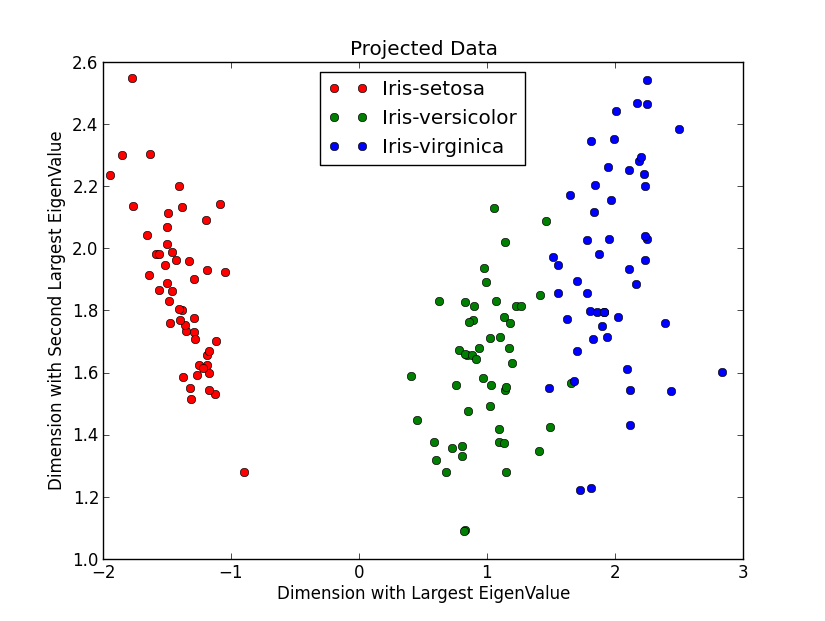
\includegraphics[width=5in,height=3.8in]{./figure_1.png}
\end{center}
(c) Discuss the ratio of the two eigenvalues found with respect to the task of classifying the data in the projected 2-dimensional space. \\
\htab Again, present the the two eigenvalues found first,
    $$ \lambda_{1} = 32.1919292,  \lambda_{2} = 0.285391043 $$
\htab And the ratio of those two eigenvalues are as follows,
    $$ r = \frac{\lambda_{1}}{\lambda_{2}} = 112.799367851 $$
    \htab Note that the horizontal coordinate axis $X_{1}$ corresponds to the dimension with $\lambda_{1}$, the vertical coordinate axis $X_{2}$ corresponds to the dimension with $\lambda_{2}$. \\
    \htab From the result of data projection in two dimension, we can see that \textbf{those three classes has tremendous distinction in the horizental coordinate} (with large eigenvalue), while the differences in the vertical coordinate (with the smaller eigenvalue). Therefore, I believe in the intuition that \textbf{the ratio of two eigenvalues $r$ shows the relative distinguishability (between two dimensions) of data objects from each other class}. And by the way, such distinguisability may come from the large between-class variance and small within-class variance.
\newpage

% 3.1.3
\subsubsection{Codes to Compute criteria $J$}
\htab We have accomplished the codes to compute $S_{w}$, $S_{B}$ and then criteria $J$ for projecting original data into $\V_{1}$ $\V_{2}$, please see getSolution\_3\_3\_, \\
\htab Within-Class Scatter Matrix:\\
$$ S_{W} = \begin{pmatrix}   
    9.31175619 &  -2.18194354\times 10^{-08} \\
    -2.18194354\times 10^{-08}   &  10.7967585  
 \end{pmatrix} $$
\htab Between-Class Scatter Matrix:\\
$$ S_{B} = \begin{pmatrix}
    299.763396  & 2.58546748\times 10^{-06}  \\
    2.58546748\times 10^{-6}  &  3.08129816  
\end{pmatrix} $$
\htab Then, we derive: \\
$$ S_{W}^{-1} S_{B} = \begin{pmatrix}
    32.1919292  &  2.78325001\times 10^{-07} \\
    3.04524474\times 10^{-07}   & 0.285391043
    \end{pmatrix} $$
\htab Finally, we have trace of $ S_{W}^{-1} S_{B} $,
$$ J = tr\{S_{W}^{-1}S_{B}\} = 32.4773202409 $$

% 3.1.4
\subsubsection{Compare to other projection}
\htab We have achieved automatically derive all combinations of two-axes projection. And use the predefined framework to work out criteria $J$ for each combination, please see getSolution\_3\_4\_, \\ 
\begin{center}
\begin{tabular} {|| c | c ||}
    \hline 
    projecting combo & criteria $J$ \\ \hline 
    $\V_{1}$, $\V_{2}$ & 32.4773202409 \\ \hline 
    Sepal Length ,  Sepal Width  & 4.3327944087 \\ \hline 
    Sepal Length ,  Petal Length  & 23.3646503713 \\ \hline 
    Sepal Length ,  Petal Width  & 13.0644017179 \\ \hline 
    Sepal Width ,  Petal Length  & 21.8610096544 \\ \hline 
    Sepal Width ,  Petal Width  & 20.3468961554 \\ \hline 
    Petal Length ,  Petal Width  & 19.7820503322 \\ \hline 
\end{tabular}
\end{center}
\htab Note that the Sepal Length,  Sepal Width, Petal Length, Petal Width are the 1st, 2nd, 3rd, 4th feature in the original input Iris data, respectively. \\
\htab It is obvious that \textbf{ the practice of projecting data into $\V_{1}$,$\V_{2}$ derived from fisher algorithm has the best outcome in maximizing between-class variance the and minimizing the within-class variance in the meanwhile}, comparing to projecting into any combination of 2-dimensional axes in original space. \\
\htab It may be generalized to a wider conclusion that for any dimension $D' (D'< n)$ ($n$ is the number of input features),  the projecting matrix $W_{n\times D'}$ figured out by fisher's algorithm are the best projection to classify data objects among all possible $D'$-dimension projection. This is for the reason that the indicator $J$ of projection from fisher algorithm's would be largest among all $D'$-dimension projection.
\newpage

% 4
\section{Cross Validation and Classification}
% 4.1
\subsection{K-Nearest Neighbours Algorithm}
% 4.1.1
\subsubsection{Implement K-NN algorithm}
\htab See the codes for implementing the K-NN algorithm. \\
\htab I also implement the min-max normalization for the original data for the reason that the KNN algorithm is vulnerable to bad scaling. (see the scaling function in KNN.py) \\
\htab In the KNN.py, the function getSolution\_4\_1\_1 is a test function for the KNN Implementation. It uses the last data of Iris datasets as the only testing data object and the rest as training dataset. 

% 4.1.2
\subsubsection{Apply Cross Validation}
\htab For 2-fold cross validation, we pick up $ k = 11 $, 
whose average cross validation test error is $ 2.66 \% $ . 
\hyperlink{twoFoldResult}{Click here to see the whole tabular result.} \\

For 5-fold cross validation, we pick up $ k = 16 $, 
whose average cross validation test error is $ 2.66 \% $ . 
\hyperlink{fiveFoldResult}{Click here to see the whole tabular result}. \\

For 10-fold cross validation, we pick up $ k = 30 $, 
whose average cross validation test error is $ 2.66 \% $ . 
\hyperlink{tenFoldResult}{Click here to see the whole tabular result}. \\

\newpage
% 4.1.3
\subsubsection{Report result of cross validation}
\textbf{2NN:} \\
2-fold CV, average error: 6.00\%  ( 4.00\%, 8.00\% )\\
5-fold CV, average error: 4.00\%  ( 3.33\%, 3.33\%, 3.33\%, 10.00\%, 0.00\% )\\
10-fold CV, average error: 4.00\%  ( 0.00\%, 6.67\%, 0.00\%, 6.67\%, 6.67\%, 0.00\%, 20.00\%, 0.00\%, 0.00\%, 0.00\% )\\
\textbf{4NN:} \\
2-fold CV, average error: 3.33\%  ( 4.00\%, 2.67\% )\\
5-fold CV, average error: 3.33\%  ( 3.33\%, 3.33\%, 0.00\%, 10.00\%, 0.00\% )\\
10-fold CV, average error: 4.00\%  ( 0.00\%, 6.67\%, 0.00\%, 6.67\%, 6.67\%, 0.00\%, 20.00\%, 0.00\%, 0.00\%, 0.00\% )\\
\textbf{6NN:} \\
2-fold CV, average error: 4.67\%  ( 5.33\%, 4.00\% )\\
5-fold CV, average error: 3.33\%  ( 3.33\%, 3.33\%, 0.00\%, 10.00\%, 0.00\% )\\
10-fold CV, average error: 3.33\%  ( 0.00\%, 6.67\%, 0.00\%, 6.67\%, 0.00\%, 0.00\%, 20.00\%, 0.00\%, 0.00\%, 0.00\% )\\
\textbf{8NN:} \\
2-fold CV, average error: 4.00\%  ( 4.00\%, 4.00\% )\\
5-fold CV, average error: 4.00\%  ( 3.33\%, 3.33\%, 3.33\%, 10.00\%, 0.00\% )\\
10-fold CV, average error: 4.00\%  ( 0.00\%, 6.67\%, 0.00\%, 6.67\%, 0.00\%, 6.67\%, 20.00\%, 0.00\%, 0.00\%, 0.00\% )\\
\textbf{10NN:} \\
2-fold CV, average error: 4.00\%  ( 4.00\%, 4.00\% )\\
5-fold CV, average error: 4.00\%  ( 3.33\%, 3.33\%, 3.33\%, 10.00\%, 0.00\% )\\
10-fold CV, average error: 4.00\%  ( 0.00\%, 6.67\%, 0.00\%, 6.67\%, 0.00\%, 6.67\%, 20.00\%, 0.00\%, 0.00\%, 0.00\% )\\
\textbf{12NN:} \\
2-fold CV, average error: 3.33\%  ( 4.00\%, 2.67\% )\\
5-fold CV, average error: 4.00\%  ( 3.33\%, 3.33\%, 3.33\%, 10.00\%, 0.00\% )\\
10-fold CV, average error: 4.00\%  ( 0.00\%, 6.67\%, 0.00\%, 6.67\%, 0.00\%, 6.67\%, 20.00\%, 0.00\%, 0.00\%, 0.00\% )\\
\textbf{14NN:} \\
2-fold CV, average error: 5.33\%  ( 5.33\%, 5.33\% )\\
5-fold CV, average error: 3.33\%  ( 3.33\%, 3.33\%, 0.00\%, 10.00\%, 0.00\% )\\
10-fold CV, average error: 4.00\%  ( 0.00\%, 6.67\%, 0.00\%, 6.67\%, 0.00\%, 6.67\%, 20.00\%, 0.00\%, 0.00\%, 0.00\% )\\
\textbf{16NN:} \\
2-fold CV, average error: 6.67\%  ( 5.33\%, 8.00\% )\\
5-fold CV, average error: 2.67\%  ( 3.33\%, 3.33\%, 0.00\%, 6.67\%, 0.00\% )\\
10-fold CV, average error: 3.33\%  ( 0.00\%, 6.67\%, 0.00\%, 6.67\%, 0.00\%, 0.00\%, 13.33\%, 6.67\%, 0.00\%, 0.00\% )\\
\textbf{18NN:} \\
2-fold CV, average error: 4.67\%  ( 2.67\%, 6.67\% )\\
5-fold CV, average error: 3.33\%  ( 3.33\%, 3.33\%, 3.33\%, 6.67\%, 0.00\% )\\
10-fold CV, average error: 4.00\%  ( 0.00\%, 6.67\%, 0.00\%, 6.67\%, 0.00\%, 6.67\%, 20.00\%, 0.00\%, 0.00\%, 0.00\% )\\
\textbf{20NN:} \\
2-fold CV, average error: 5.33\%  ( 5.33\%, 5.33\% )\\
5-fold CV, average error: 4.00\%  ( 6.67\%, 3.33\%, 0.00\%, 10.00\%, 0.00\% )\\
10-fold CV, average error: 4.67\%  ( 0.00\%, 6.67\%, 0.00\%, 6.67\%, 6.67\%, 6.67\%, 20.00\%, 0.00\%, 0.00\%, 0.00\% )\\
\textbf{22NN:} \\
2-fold CV, average error: 6.00\%  ( 5.33\%, 6.67\% )\\
5-fold CV, average error: 4.67\%  ( 6.67\%, 3.33\%, 3.33\%, 10.00\%, 0.00\% )\\
10-fold CV, average error: 4.00\%  ( 0.00\%, 6.67\%, 0.00\%, 6.67\%, 6.67\%, 0.00\%, 20.00\%, 0.00\%, 0.00\%, 0.00\% )\\
\textbf{24NN:} \\
2-fold CV, average error: 6.67\%  ( 5.33\%, 8.00\% )\\
5-fold CV, average error: 4.67\%  ( 6.67\%, 3.33\%, 3.33\%, 10.00\%, 0.00\% )\\
10-fold CV, average error: 3.33\%  ( 0.00\%, 6.67\%, 0.00\%, 6.67\%, 0.00\%, 0.00\%, 20.00\%, 0.00\%, 0.00\%, 0.00\% )\\
\textbf{26NN:} \\
2-fold CV, average error: 8.00\%  ( 8.00\%, 8.00\% )\\
5-fold CV, average error: 4.00\%  ( 6.67\%, 3.33\%, 3.33\%, 6.67\%, 0.00\% )\\
10-fold CV, average error: 4.67\%  ( 6.67\%, 6.67\%, 0.00\%, 6.67\%, 6.67\%, 0.00\%, 20.00\%, 0.00\%, 0.00\%, 0.00\% )\\
\textbf{28NN:} \\
2-fold CV, average error: 9.33\%  ( 9.33\%, 9.33\% )\\
5-fold CV, average error: 4.00\%  ( 6.67\%, 3.33\%, 3.33\%, 6.67\%, 0.00\% )\\
10-fold CV, average error: 4.00\%  ( 0.00\%, 6.67\%, 0.00\%, 6.67\%, 6.67\%, 0.00\%, 20.00\%, 0.00\%, 0.00\%, 0.00\% )\\
\textbf{30NN:} \\
2-fold CV, average error: 11.33\%  ( 12.00\%, 10.67\% )\\
5-fold CV, average error: 4.00\%  ( 3.33\%, 3.33\%, 3.33\%, 10.00\%, 0.00\% )\\
10-fold CV, average error: 2.67\%  ( 0.00\%, 6.67\%, 0.00\%, 6.67\%, 0.00\%, 0.00\%, 13.33\%, 0.00\%, 0.00\%, 0.00\% )\\
\textbf{32NN:} \\
2-fold CV, average error: 11.33\%  ( 12.00\%, 10.67\% )\\
5-fold CV, average error: 4.00\%  ( 3.33\%, 3.33\%, 3.33\%, 10.00\%, 0.00\% )\\
10-fold CV, average error: 4.00\%  ( 0.00\%, 6.67\%, 0.00\%, 6.67\%, 0.00\%, 6.67\%, 13.33\%, 6.67\%, 0.00\%, 0.00\% )\\
\textbf{34NN:} \\
2-fold CV, average error: 12.00\%  ( 13.33\%, 10.67\% )\\
5-fold CV, average error: 4.00\%  ( 3.33\%, 3.33\%, 3.33\%, 10.00\%, 0.00\% )\\
10-fold CV, average error: 4.00\%  ( 0.00\%, 6.67\%, 0.00\%, 6.67\%, 0.00\%, 6.67\%, 13.33\%, 6.67\%, 0.00\%, 0.00\% )\\
\textbf{36NN:} \\
2-fold CV, average error: 12.00\%  ( 13.33\%, 10.67\% )\\
5-fold CV, average error: 5.33\%  ( 10.00\%, 3.33\%, 3.33\%, 10.00\%, 0.00\% )\\
10-fold CV, average error: 4.00\%  ( 0.00\%, 6.67\%, 0.00\%, 6.67\%, 0.00\%, 6.67\%, 13.33\%, 6.67\%, 0.00\%, 0.00\% )\\
\textbf{38NN:} \\
2-fold CV, average error: 12.00\%  ( 12.00\%, 12.00\% )\\
5-fold CV, average error: 4.67\%  ( 6.67\%, 3.33\%, 3.33\%, 10.00\%, 0.00\% )\\
10-fold CV, average error: 5.33\%  ( 0.00\%, 6.67\%, 0.00\%, 6.67\%, 0.00\%, 20.00\%, 13.33\%, 6.67\%, 0.00\%, 0.00\% )\\

\newpage
% 4.1.4
\subsubsection{Explain optimal error decreases with fold number}
    
% 4.1.5
\subsubsection{Explain optimal $k$ decreases with fold number}

% 4.1.6
\subsubsection{Listing of programs and solutions}
\begin{verbatim}
KNN.py
  class
    KNNClassifier
    CrossValidation

  member
    __init__ [KNNClassifier]
    getFeatureVector [KNNClassifier]
    getLabel [KNNClassifier]
    getEuclidianDistance [KNNClassifier]
    getDistance [KNNClassifier]
    getKNearestNeighbours [KNNClassifier]
    majorityVoting [KNNClassifier]
    run [KNNClassifier]
    __init__ [CrossValidation]
    getRandomGroup [CrossValidation]
    getError [CrossValidation]
    run [CrossValidation]

  function
    printMatrix
    classMapping
    readMatrix
    scaling
    getSolution_4_1_1_
    getSolution_4_1_2_
    getSolution_4_1_3_
    main
\end{verbatim}

\newpage

% appendix
% A. proof for linearity 
\appendix
\section{Supplementary proof for 1.1}
\hypertarget{Linearity}{}
\subsection{ Proof of linearity of $\mu_{x+y}$ }
\htab Based on definition of expectation, we have
    $$ \mu_{x+y} = \dinfint (x+y) P(x,y) dx dy \eqno (1) $$
    $$ \mu_{x} = \infint x P(x) dx \eqno (2) $$
    $$ \mu_{y} = \infint y P(y) dy \eqno (3) $$
\htab Note that we use $\mu$ as abbreviation of expectation of certain random variable. \\
\htab Then we start manipulating $\mu_{x+y}$ from $(1)$
$$ 
\begin{aligned}
    \mu_{x+y} & = \dinfint \Big[ xP(x,y) + yP(x,y) \Big] dx dy \\
    & = \dinfint xP(x,y) dx dy + \dinfint yP(x,y) dx dy \\
    & = \infint xP(x) dx + \infint yP(y) dy 
\end{aligned}
\eqno (4) $$
\htab Note that last derivation above is based on sum rule of probability. \\
\htab By taking $(2)$ and $(3)$ for $(4)$, we solve the proof
    $$ \mu_{x+y }= \mu_{x} + \mu_{y} \eqno (5) $$

% B. proof of derivation of Gaussian distribution
\section{Supplementary proofs for 1.3}
\hypertarget{Derivation}{}
\subsection{Specifics of first derivative to likelihood} 
\hypertarget{DerivationB}{}
\subsection{Specifics of second derivative to likelihood}
\newpage


% C. result for Cross validation
\section{Cross Validation result}
\hypertarget{twoFoldResult}{}
\subsection{2-fold cross validation}
\begin{center}
    \begin{tabular} {|| c | c | c ||}
        \hline
        item name & average error & error of each group \\ \hline
       2NN 2-fold CV & 6.00\% & ( 4.00\%, 8.00\% ) \\ \hline
        3NN 2-fold CV & 4.67\% & ( 5.33\%, 4.00\% ) \\ \hline
        4NN 2-fold CV & 3.33\% & ( 4.00\%, 2.67\% ) \\ \hline
        5NN 2-fold CV & 4.67\% & ( 4.00\%, 5.33\% ) \\ \hline
        6NN 2-fold CV & 4.67\% & ( 5.33\%, 4.00\% ) \\ \hline
        7NN 2-fold CV & 4.67\% & ( 5.33\%, 4.00\% ) \\ \hline
        8NN 2-fold CV & 4.00\% & ( 4.00\%, 4.00\% ) \\ \hline
        9NN 2-fold CV & 4.67\% & ( 4.00\%, 5.33\% ) \\ \hline
        10NN 2-fold CV & 4.00\% & ( 4.00\%, 4.00\% ) \\ \hline
        11NN 2-fold CV & 2.67\% & ( 4.00\%, 1.33\% ) \\ \hline
        12NN 2-fold CV & 3.33\% & ( 4.00\%, 2.67\% ) \\ \hline
        13NN 2-fold CV & 4.00\% & ( 5.33\%, 2.67\% ) \\ \hline
        14NN 2-fold CV & 5.33\% & ( 5.33\%, 5.33\% ) \\ \hline
        15NN 2-fold CV & 4.67\% & ( 5.33\%, 4.00\% ) \\ \hline
        16NN 2-fold CV & 6.67\% & ( 5.33\%, 8.00\% ) \\ \hline
        17NN 2-fold CV & 6.67\% & ( 6.67\%, 6.67\% ) \\ \hline
        18NN 2-fold CV & 4.67\% & ( 2.67\%, 6.67\% ) \\ \hline
        19NN 2-fold CV & 5.33\% & ( 5.33\%, 5.33\% ) \\ \hline
        20NN 2-fold CV & 5.33\% & ( 5.33\%, 5.33\% ) \\ \hline
        21NN 2-fold CV & 5.33\% & ( 5.33\%, 5.33\% ) \\ \hline
        22NN 2-fold CV & 6.00\% & ( 5.33\%, 6.67\% ) \\ \hline
        23NN 2-fold CV & 6.00\% & ( 5.33\%, 6.67\% ) \\ \hline
        24NN 2-fold CV & 6.67\% & ( 5.33\%, 8.00\% ) \\ \hline
        25NN 2-fold CV & 6.67\% & ( 5.33\%, 8.00\% ) \\ \hline
        26NN 2-fold CV & 8.00\% & ( 8.00\%, 8.00\% ) \\ \hline
        27NN 2-fold CV & 8.67\% & ( 8.00\%, 9.33\% ) \\ \hline
        28NN 2-fold CV & 9.33\% & ( 9.33\%, 9.33\% ) \\ \hline
        29NN 2-fold CV & 9.33\% & ( 10.67\%, 8.00\% ) \\ \hline
        30NN 2-fold CV & 11.33\% & ( 12.00\%, 10.67\% ) \\ \hline
        31NN 2-fold CV & 11.33\% & ( 12.00\%, 10.67\% ) \\ \hline
        32NN 2-fold CV & 11.33\% & ( 12.00\%, 10.67\% ) \\ \hline
        33NN 2-fold CV & 12.00\% & ( 13.33\%, 10.67\% ) \\ \hline
        34NN 2-fold CV & 12.00\% & ( 13.33\%, 10.67\% ) \\ \hline
        35NN 2-fold CV & 12.00\% & ( 13.33\%, 10.67\% ) \\ \hline
        36NN 2-fold CV & 12.00\% & ( 13.33\%, 10.67\% ) \\ \hline
        37NN 2-fold CV & 12.00\% & ( 13.33\%, 10.67\% ) \\ \hline
        38NN 2-fold CV & 12.00\% & ( 12.00\%, 12.00\% ) \\ \hline
        39NN 2-fold CV & 12.67\% & ( 13.33\%, 12.00\% ) \\ \hline 
    \end{tabular}
\end{center}
\newpage
\hypertarget{fiveFoldResult}{}
\subsection{5-fold cross validation}
\begin{center}
    \begin{tabular} {|| c | c | c ||}
        \hline
        item name & average error & error of each group \\ \hline
        2NN 5-fold CV & 4.00\% & ( 3.33\%, 3.33\%, 3.33\%, 10.00\%, 0.00\% ) \\ \hline
        3NN 5-fold CV & 4.67\% & ( 3.33\%, 3.33\%, 6.67\%, 10.00\%, 0.00\% ) \\ \hline
        4NN 5-fold CV & 3.33\% & ( 3.33\%, 3.33\%, 0.00\%, 10.00\%, 0.00\% ) \\ \hline
        5NN 5-fold CV & 4.00\% & ( 3.33\%, 3.33\%, 3.33\%, 10.00\%, 0.00\% ) \\ \hline
        6NN 5-fold CV & 3.33\% & ( 3.33\%, 3.33\%, 0.00\%, 10.00\%, 0.00\% ) \\ \hline
        7NN 5-fold CV & 4.00\% & ( 3.33\%, 3.33\%, 3.33\%, 10.00\%, 0.00\% ) \\ \hline
        8NN 5-fold CV & 4.00\% & ( 3.33\%, 3.33\%, 3.33\%, 10.00\%, 0.00\% ) \\ \hline
        9NN 5-fold CV & 4.00\% & ( 3.33\%, 3.33\%, 3.33\%, 10.00\%, 0.00\% ) \\ \hline
        10NN 5-fold CV & 4.00\% & ( 3.33\%, 3.33\%, 3.33\%, 10.00\%, 0.00\% ) \\ \hline
        11NN 5-fold CV & 4.00\% & ( 3.33\%, 3.33\%, 3.33\%, 10.00\%, 0.00\% ) \\ \hline
        12NN 5-fold CV & 4.00\% & ( 3.33\%, 3.33\%, 3.33\%, 10.00\%, 0.00\% ) \\ \hline
        13NN 5-fold CV & 4.00\% & ( 3.33\%, 3.33\%, 3.33\%, 10.00\%, 0.00\% ) \\ \hline
        14NN 5-fold CV & 3.33\% & ( 3.33\%, 3.33\%, 0.00\%, 10.00\%, 0.00\% ) \\ \hline
        15NN 5-fold CV & 2.67\% & ( 3.33\%, 3.33\%, 0.00\%, 6.67\%, 0.00\% ) \\ \hline
        16NN 5-fold CV & 2.67\% & ( 3.33\%, 3.33\%, 0.00\%, 6.67\%, 0.00\% ) \\ \hline
        17NN 5-fold CV & 4.00\% & ( 3.33\%, 3.33\%, 6.67\%, 6.67\%, 0.00\% ) \\ \hline
        18NN 5-fold CV & 3.33\% & ( 3.33\%, 3.33\%, 3.33\%, 6.67\%, 0.00\% ) \\ \hline
        19NN 5-fold CV & 5.33\% & ( 6.67\%, 3.33\%, 6.67\%, 10.00\%, 0.00\% ) \\ \hline
        20NN 5-fold CV & 4.00\% & ( 6.67\%, 3.33\%, 0.00\%, 10.00\%, 0.00\% ) \\ \hline
        21NN 5-fold CV & 5.33\% & ( 6.67\%, 3.33\%, 6.67\%, 10.00\%, 0.00\% ) \\ \hline
        22NN 5-fold CV & 4.67\% & ( 6.67\%, 3.33\%, 3.33\%, 10.00\%, 0.00\% ) \\ \hline
        23NN 5-fold CV & 4.67\% & ( 6.67\%, 3.33\%, 6.67\%, 6.67\%, 0.00\% ) \\ \hline
        24NN 5-fold CV & 4.67\% & ( 6.67\%, 3.33\%, 3.33\%, 10.00\%, 0.00\% ) \\ \hline
        25NN 5-fold CV & 5.33\% & ( 6.67\%, 3.33\%, 6.67\%, 10.00\%, 0.00\% ) \\ \hline
        26NN 5-fold CV & 4.00\% & ( 6.67\%, 3.33\%, 3.33\%, 6.67\%, 0.00\% ) \\ \hline
        27NN 5-fold CV & 4.00\% & ( 6.67\%, 3.33\%, 3.33\%, 6.67\%, 0.00\% ) \\ \hline
        28NN 5-fold CV & 4.00\% & ( 6.67\%, 3.33\%, 3.33\%, 6.67\%, 0.00\% ) \\ \hline
        29NN 5-fold CV & 4.00\% & ( 6.67\%, 3.33\%, 3.33\%, 6.67\%, 0.00\% ) \\ \hline
        30NN 5-fold CV & 4.00\% & ( 3.33\%, 3.33\%, 3.33\%, 10.00\%, 0.00\% ) \\ \hline
        31NN 5-fold CV & 4.00\% & ( 3.33\%, 3.33\%, 3.33\%, 10.00\%, 0.00\% ) \\ \hline
        32NN 5-fold CV & 4.00\% & ( 3.33\%, 3.33\%, 3.33\%, 10.00\%, 0.00\% ) \\ \hline
        33NN 5-fold CV & 4.00\% & ( 3.33\%, 3.33\%, 3.33\%, 10.00\%, 0.00\% ) \\ \hline
        34NN 5-fold CV & 4.00\% & ( 3.33\%, 3.33\%, 3.33\%, 10.00\%, 0.00\% ) \\ \hline
        35NN 5-fold CV & 5.33\% & ( 10.00\%, 3.33\%, 3.33\%, 10.00\%, 0.00\% ) \\ \hline
        36NN 5-fold CV & 5.33\% & ( 10.00\%, 3.33\%, 3.33\%, 10.00\%, 0.00\% ) \\ \hline
        37NN 5-fold CV & 5.33\% & ( 10.00\%, 3.33\%, 3.33\%, 10.00\%, 0.00\% ) \\ \hline
        38NN 5-fold CV & 4.67\% & ( 6.67\%, 3.33\%, 3.33\%, 10.00\%, 0.00\% ) \\ \hline
        39NN 5-fold CV & 4.67\% & ( 6.67\%, 3.33\%, 3.33\%, 10.00\%, 0.00\% ) \\ \hline
    \end{tabular}
\end{center}
\newpage
\hypertarget{tenFoldResult}{}
\subsection{10-fold cross validation}
\begin{center}
    \begin{tabular} {|| c | c | c ||}
        \hline
        item name & AVE & error of each group \\ \hline
2NN 10-fold CV & 4.00\% & ( 0.00\%, 6.67\%, 0.00\%, 6.67\%, 6.67\%, 0.00\%, 20.00\%, 0.00\%, 0.00\%, 0.00\% ) \\ \hline
3NN 10-fold CV & 4.67\% & ( 0.00\%, 6.67\%, 0.00\%, 6.67\%, 13.33\%, 0.00\%, 20.00\%, 0.00\%, 0.00\%, 0.00\% ) \\ \hline
4NN 10-fold CV & 4.00\% & ( 0.00\%, 6.67\%, 0.00\%, 6.67\%, 6.67\%, 0.00\%, 20.00\%, 0.00\%, 0.00\%, 0.00\% ) \\ \hline
5NN 10-fold CV & 4.67\% & ( 0.00\%, 6.67\%, 0.00\%, 6.67\%, 6.67\%, 6.67\%, 20.00\%, 0.00\%, 0.00\%, 0.00\% ) \\ \hline
6NN 10-fold CV & 3.33\% & ( 0.00\%, 6.67\%, 0.00\%, 6.67\%, 0.00\%, 0.00\%, 20.00\%, 0.00\%, 0.00\%, 0.00\% ) \\ \hline
7NN 10-fold CV & 4.00\% & ( 0.00\%, 6.67\%, 0.00\%, 6.67\%, 0.00\%, 6.67\%, 20.00\%, 0.00\%, 0.00\%, 0.00\% ) \\ \hline
8NN 10-fold CV & 4.00\% & ( 0.00\%, 6.67\%, 0.00\%, 6.67\%, 0.00\%, 6.67\%, 20.00\%, 0.00\%, 0.00\%, 0.00\% ) \\ \hline
9NN 10-fold CV & 4.00\% & ( 0.00\%, 6.67\%, 0.00\%, 0.00\%, 6.67\%, 6.67\%, 20.00\%, 0.00\%, 0.00\%, 0.00\% ) \\ \hline
10NN 10-fold CV & 4.00\% & ( 0.00\%, 6.67\%, 0.00\%, 6.67\%, 0.00\%, 6.67\%, 20.00\%, 0.00\%, 0.00\%, 0.00\% ) \\ \hline
11NN 10-fold CV & 4.67\% & ( 0.00\%, 6.67\%, 0.00\%, 6.67\%, 6.67\%, 6.67\%, 20.00\%, 0.00\%, 0.00\%, 0.00\% ) \\ \hline
12NN 10-fold CV & 4.00\% & ( 0.00\%, 6.67\%, 0.00\%, 6.67\%, 0.00\%, 6.67\%, 20.00\%, 0.00\%, 0.00\%, 0.00\% ) \\ \hline
13NN 10-fold CV & 4.00\% & ( 0.00\%, 6.67\%, 0.00\%, 6.67\%, 0.00\%, 6.67\%, 20.00\%, 0.00\%, 0.00\%, 0.00\% ) \\ \hline
14NN 10-fold CV & 4.00\% & ( 0.00\%, 6.67\%, 0.00\%, 6.67\%, 0.00\%, 6.67\%, 20.00\%, 0.00\%, 0.00\%, 0.00\% ) \\ \hline
15NN 10-fold CV & 3.33\% & ( 0.00\%, 6.67\%, 0.00\%, 6.67\%, 0.00\%, 6.67\%, 13.33\%, 0.00\%, 0.00\%, 0.00\% ) \\ \hline
16NN 10-fold CV & 3.33\% & ( 0.00\%, 6.67\%, 0.00\%, 6.67\%, 0.00\%, 0.00\%, 13.33\%, 6.67\%, 0.00\%, 0.00\% ) \\ \hline
17NN 10-fold CV & 3.33\% & ( 0.00\%, 6.67\%, 0.00\%, 6.67\%, 0.00\%, 6.67\%, 13.33\%, 0.00\%, 0.00\%, 0.00\% ) \\ \hline
18NN 10-fold CV & 4.00\% & ( 0.00\%, 6.67\%, 0.00\%, 6.67\%, 0.00\%, 6.67\%, 20.00\%, 0.00\%, 0.00\%, 0.00\% ) \\ \hline
19NN 10-fold CV & 4.67\% & ( 0.00\%, 6.67\%, 0.00\%, 6.67\%, 6.67\%, 6.67\%, 20.00\%, 0.00\%, 0.00\%, 0.00\% ) \\ \hline
20NN 10-fold CV & 4.67\% & ( 0.00\%, 6.67\%, 0.00\%, 6.67\%, 6.67\%, 6.67\%, 20.00\%, 0.00\%, 0.00\%, 0.00\% ) \\ \hline
21NN 10-fold CV & 4.67\% & ( 0.00\%, 6.67\%, 0.00\%, 6.67\%, 6.67\%, 6.67\%, 20.00\%, 0.00\%, 0.00\%, 0.00\% ) \\ \hline
22NN 10-fold CV & 4.00\% & ( 0.00\%, 6.67\%, 0.00\%, 6.67\%, 6.67\%, 0.00\%, 20.00\%, 0.00\%, 0.00\%, 0.00\% ) \\ \hline
23NN 10-fold CV & 4.67\% & ( 0.00\%, 6.67\%, 0.00\%, 6.67\%, 6.67\%, 6.67\%, 20.00\%, 0.00\%, 0.00\%, 0.00\% ) \\ \hline
24NN 10-fold CV & 3.33\% & ( 0.00\%, 6.67\%, 0.00\%, 6.67\%, 0.00\%, 0.00\%, 20.00\%, 0.00\%, 0.00\%, 0.00\% ) \\ \hline
25NN 10-fold CV & 5.33\% & ( 6.67\%, 6.67\%, 0.00\%, 6.67\%, 6.67\%, 6.67\%, 20.00\%, 0.00\%, 0.00\%, 0.00\% ) \\ \hline
26NN 10-fold CV & 4.67\% & ( 6.67\%, 6.67\%, 0.00\%, 6.67\%, 6.67\%, 0.00\%, 20.00\%, 0.00\%, 0.00\%, 0.00\% ) \\ \hline
27NN 10-fold CV & 5.33\% & ( 6.67\%, 6.67\%, 0.00\%, 6.67\%, 6.67\%, 6.67\%, 20.00\%, 0.00\%, 0.00\%, 0.00\% ) \\ \hline
28NN 10-fold CV & 4.00\% & ( 0.00\%, 6.67\%, 0.00\%, 6.67\%, 6.67\%, 0.00\%, 20.00\%, 0.00\%, 0.00\%, 0.00\% ) \\ \hline
29NN 10-fold CV & 4.00\% & ( 0.00\%, 6.67\%, 0.00\%, 6.67\%, 6.67\%, 0.00\%, 20.00\%, 0.00\%, 0.00\%, 0.00\% ) \\ \hline
30NN 10-fold CV & 2.67\% & ( 0.00\%, 6.67\%, 0.00\%, 6.67\%, 0.00\%, 0.00\%, 13.33\%, 0.00\%, 0.00\%, 0.00\% ) \\ \hline
31NN 10-fold CV & 4.00\% & ( 6.67\%, 6.67\%, 0.00\%, 6.67\%, 0.00\%, 6.67\%, 13.33\%, 0.00\%, 0.00\%, 0.00\% ) \\ \hline
32NN 10-fold CV & 4.00\% & ( 0.00\%, 6.67\%, 0.00\%, 6.67\%, 0.00\%, 6.67\%, 13.33\%, 6.67\%, 0.00\%, 0.00\% ) \\ \hline
33NN 10-fold CV & 4.00\% & ( 0.00\%, 6.67\%, 0.00\%, 6.67\%, 0.00\%, 6.67\%, 13.33\%, 6.67\%, 0.00\%, 0.00\% ) \\ \hline
34NN 10-fold CV & 4.00\% & ( 0.00\%, 6.67\%, 0.00\%, 6.67\%, 0.00\%, 6.67\%, 13.33\%, 6.67\%, 0.00\%, 0.00\% ) \\ \hline
35NN 10-fold CV & 4.00\% & ( 0.00\%, 6.67\%, 0.00\%, 6.67\%, 0.00\%, 6.67\%, 13.33\%, 6.67\%, 0.00\%, 0.00\% ) \\ \hline
36NN 10-fold CV & 4.00\% & ( 0.00\%, 6.67\%, 0.00\%, 6.67\%, 0.00\%, 6.67\%, 13.33\%, 6.67\%, 0.00\%, 0.00\% ) \\ \hline
37NN 10-fold CV & 4.00\% & ( 0.00\%, 6.67\%, 0.00\%, 6.67\%, 0.00\%, 6.67\%, 13.33\%, 6.67\%, 0.00\%, 0.00\% ) \\ \hline
38NN 10-fold CV & 5.33\% & ( 0.00\%, 6.67\%, 0.00\%, 6.67\%, 0.00\%, 20.00\%, 13.33\%, 6.67\%, 0.00\%, 0.00\% ) \\ \hline
39NN 10-fold CV & 5.33\% & ( 13.33\%, 6.67\%, 0.00\%, 6.67\%, 0.00\%, 6.67\%, 13.33\%, 6.67\%, 0.00\%, 0.00\% ) \\ \hline
    \end{tabular}
\end{center}
\newpage
\end{document}
